\documentclass[11pt]{book} 
\RequirePackage{silence}
\WarningFilter{remreset}{The remreset package}

\title{MAT247 - Probability with Computer Applications}
\author{Callum Cassidy-Nolan}

% Packages
\usepackage{amsmath}
\usepackage{amssymb}
\usepackage{mathtools}
\usepackage{xcolor}
\usepackage{amsthm}
\usepackage{thmtools}
\usepackage{amsfonts}
\usepackage{geometry}
\usepackage{gauss}
\usepackage{pifont}
\usepackage{hyperref}
\usepackage{witharrows}
\usepackage{cleveref}
\usepackage{tikz}
\usepackage{bm}
\usepackage{todonotes}
\usepackage{enumitem}
\usepackage{mdframed}
\usetikzlibrary{patterns,angles,quotes,decorations.pathreplacing}
\hypersetup{
    colorlinks=true, %set true if you want colored links
    linktoc=all,     %set to all if you want both sections and subsections linked
    linkcolor=blue,  %choose some color if you want links to stand out
}


% BlackSquare for proofs
\renewcommand{\qedsymbol}{$\blacksquare$}

\theoremstyle{definition}

% Matricies
\newcommand\mat[2][b]{\begin{#1matrix}#2\end{#1matrix}}

% Augmented matrix
\makeatletter
\renewcommand*\env@matrix[1][*\c@MaxMatrixCols c]{%
  \hskip -\arraycolsep
  \let\@ifnextchar\new@ifnextchar
  \array{#1}}
\makeatother

% Modular Arithmetic
\newcommand{\Mod}[1]{\ (\mathrm{mod}\ #1)}

% Automatic Parenthesis scaling
\delimitershortfall-1sp
\usepackage{mleftright}
\mleftright % make \left & \right behave like \mleft & \mright

% Theorems
\newtheoremstyle{break}
  {\topsep}{\topsep}%
  {\itshape}{}%
  {\bfseries}{}%
  {\newline}{}%

\theoremstyle{break}

\newtheorem{remark}{Remark}[section]

\newtheorem{ver}{Verfication}[section]

\newtheorem{ex}{Exercise}[section]

\newtheorem{eg}{Example}[section]

% definition env
\newmdtheoremenv{defn}{Definition}

% Note env
\newmdtheoremenv{nt}{Note}

% definition env no num
\newtheorem*{defnnonum}{Definition}

% theorem envs
\newtheorem{thm}{Theorem}

% theorem envs without counter

\newtheorem{propo}[thm]{Proposition}

\newtheorem{crly}[thm]{Corollary}

\newtheorem{lemma}[thm]{Lemma}

\newtheorem{axiom}[thm]{Axiom}

\newtheorem*{thmnonum}{Theorem}

\newtheorem*{propononum}{Proposition}

\newtheorem*{crlynonum}{Corollary}

\newtheorem*{lemmanonum}{Lemma}

\newtheorem*{axiomnonum}{Axiom}


\newtheorem{note}{Note}[section]

\newtheorem{mnote}[note]{Note}

\newtheorem*{notation}{Notation}
    % warning env
\newtheorem*{warning}{Warning}

% So todo's don't get cut off
\setlength{\marginparwidth}{3cm}

% Define cuboids
\tikzset{
  annotated cuboid/.pic={
    \tikzset{%
      every edge quotes/.append style={midway, auto},
      /cuboid/.cd,
      #1
    }
    \draw [every edge/.append style={pic actions, densely dashed, opacity=.5}, pic actions]
    (0,0,0) coordinate (o) -- ++(-\cubescale*\cubex,0,0) coordinate (a) -- ++(0,-\cubescale*\cubey,0) coordinate (b) edge coordinate [pos=1] (g) ++(0,0,-\cubescale*\cubez)  -- ++(\cubescale*\cubex,0,0) coordinate (c) -- cycle
    (o) -- ++(0,0,-\cubescale*\cubez) coordinate (d) -- ++(0,-\cubescale*\cubey,0) coordinate (e) edge (g) -- (c) -- cycle
    (o) -- (a) -- ++(0,0,-\cubescale*\cubez) coordinate (f) edge (g) -- (d) -- cycle;
    \path [every edge/.append style={pic actions, |-|}]
    (b) +(0,-5pt) coordinate (b1) edge ["\cubex \cubeunits"'] (b1 -| c)
    (b) +(-5pt,0) coordinate (b2) edge ["\cubey \cubeunits"] (b2 |- a)
    (c) +(3.5pt,-3.5pt) coordinate (c2) edge ["\cubez \cubeunits"'] ([xshift=3.5pt,yshift=-3.5pt]e)
    ;
  },
  /cuboid/.search also={/tikz},
  /cuboid/.cd,
  width/.store in=\cubex,
  height/.store in=\cubey,
  depth/.store in=\cubez,
  units/.store in=\cubeunits,
  scale/.store in=\cubescale,
  width=10,
  height=10,
  depth=10,
  units=cm,
  scale=.1,
}

% highlighting shortcuts
\newcommand{\hlimpo}[1]{\textcolor{red}{\textbf{#1}}}
\newcommand{\hlwarn}[1]{\textcolor{yellow}{\textbf{#1}}}
\newcommand{\hldefn}[1]{\textcolor{blue}{\index{#1}\textbf{#1}}}
\newcommand{\hlnotea}[1]{\textcolor{green}{\textbf{#1}}}
\newcommand{\hlnoteb}[1]{\textcolor{cyan}{\textbf{#1}}}
\newcommand{\hlb}[2]{\colorbox{#1!30!background}{#2}}
\newcommand{\hlbnotea}[1]{\hlb{green}{#1}}
\newcommand{\hlbnoteb}[1]{\hlb{cyan}{#1}}
\newcommand{\hlbnotec}[1]{\hlb{yellow}{#1}}
\newcommand{\hlbnoted}[1]{\hlb{magenta}{#1}}
\newcommand{\hlbnotee}[1]{\hlb{red}{#1}}
\newcommand{\WTP}{\textcolor{bwhite}{WTP} }
\newcommand{\WTS}{\textcolor{bwhite}{WTS} }



\begin{document}

\maketitle

\tableofcontents

\renewcommand{\listtheoremname}{List of Definitions}
\listoftheorems[ignoreall,show={defn}]


\renewcommand{\listtheoremname}{\textsl{List of Theorems}}
\listoftheorems[ignoreall,
show={axiom,lemma,thm,crly,propo}
]


\chapter{Lecture 1}%
\label{chp:lecture_1}
% chapter lecture_1

\section{Stats vs Probability}%
\label{sec:stats_vs_probability}
% subsection stats_vs_probability

\underline{Statistics} 
\begin{itemize}
    \item Reverse Probability
    \item Making observations and then based on probability we describe the original model
    \item Critique whether a model is correct 
\end{itemize}
\underline{Probability} 
\begin{itemize}
    \item How likely based on a theoretical situation, for example a coin toss has a 50/50 chance of one of the outcomes.
    \item We know all the parameters.
\end{itemize}

% subsection stats_vs_probability (end)

\section{To do Well}%
\label{sec:to_do_well}
% section to_do_well

\begin{itemize}
    \item Understand the formulas
    \item Make sure to the hard questions
    \item Office hours in HS 386
\end{itemize}

% section to_do_well (end)

\newpage

\section{Useful Terminology}%
\label{sec:useful_terminology}
% section useful_terminology

\begin{defn}[Random Experiment]\index{Random Experiment}\label{defn:random_experiment}
    A process of gathering data or observations. We can perform the experiment multiple times so long as the conditions aren't changed and the outcome of each experiment is random, we don't know what the result will be, though we know the set of possible outcomes. 
\end{defn}

\underline{Examples} 

\begin{itemize}
    \item Rolling a die, and observing the number on the top face. 
    \item Rolling $n$ dice and observing the resulting pair of numbers. 
    \item Drawing 3 cards from a deck of cards
    \item Asking a professor how old they are
\end{itemize}

\begin{defn}[Sample Space]\index{Sample Space}\label{defn:sample_space}
    This is the set of all possible outcomes/results from a random experiment , we denote this set as
    \[
    \Omega \text{ or } S
    \]
    The sample space depends on the outcome of interest.
\end{defn}

\begin{nt}
    If our outcome of interest is say, whether after flipping a coin it is heads or tails, we don't care how many times it turned in the air before landing on the ground.
\end{nt}

\begin{enumerate}
    \item [\textbf{Examples}] 
    \item $S = \left\{ n \in \mathbb{N} : 1 \le  n \le 20 \right\} $.  All the faces of the dice.
    \item $\Omega _{1} = \left\{ \text{ True } , \text{ False } \right\} $ 
    \item $\Omega _{2} = \mathbb{R} ^{\ge 0} $. If they are precise in their measurement, though more likely to any hour between 0 and 10. 
\end{enumerate}

\begin{defn}[Event]\index{Event}\label{defn:event}
    Any subset of our sample space of interest. 
    \begin{itemize}
        \item Simple Event: One with exactly one outcome
        \item Compound Event: One with multiple outcomes 
    \end{itemize}
\end{defn}

    \begin{itemize}
        \item [\textbf{Simple Event}] 
        \item flipping a coin, and observing whether it has landed on it's edge (that's possible!)
        \item [\textbf{Compound Event}] 
        \item flipping 3 coins, and observing whether at least one has landed on it's edge. 
    \end{itemize}

\begin{defn}[Complement]\index{Complement}\label{defn:complement}
    The \underline{complement} of an event A is the event consisting of outcome that are nto in A. We denote this as $A^{c} $ .\\
    \textbf{For example:} the complement of our previous example, that would be if no, coin has landed on it's edge.
\end{defn}

\begin{defn}[Union]\index{Union}\label{defn:union}
    The union of two events $A \text{ and } B$ is the event consisting of outcomes in $A $  or $B$ or both. Denoted as $A\cup B$ 
    \begin{itemize}
        \item The union of events is usually said as $A$ or $B$ 
        \item Observe $AUA^{c} = \Omega $  
    \end{itemize}
\end{defn}

\begin{defn}[Intersection]\index{Intersection}\label{defn:intersection}
    The intersection of two events $A \text{ and } B$ is the event consisting of outcomes in both $A \text{ and } B$, written as $A\cap C$ 
    \begin{itemize}
        \item The intersection of events is described by $A \text{ and } B$ 
        \item We see $A\cap A^{c} = \emptyset $ 
    \end{itemize}
\end{defn}

\begin{defn}[Disjoint]\index{Disjoint}\label{defn:disjoint}
    events $A \text{ and } B$ are disjoint, if they have no overlapping events , that is $A\cap B= \emptyset $ 
\end{defn}

% section useful_terminology (end)

\section{Event Laws}%
\label{sec:event_laws}
% section event_laws

\begin{itemize}
    \item Commutative Law: $A \cup B= B\cup A$ 
    \item Associative Law:
        \begin{gather*}
            \left( A\cup B \right) \cup C = A\cup \left( B\cup C \right) \\
            \left( A \cap B \right) \cap C = A \cap \left( B\cap C \right) 
        \end{gather*}
    \item Distributive Law: $A \cap \left( B\cup C \right) = \left( A\cap B \right) \cup \left( A\cap C \right) $ (This one will be useful for proving $P\left(A\cup B\cup C\right) = P\left(A\right)  + P\left(B\right)  + \ldots  +  P\left(A\cap B\cap C\right) $ )
\end{itemize}

% section event_laws (end)

\section{Mutually Exclusive}%
\label{sec:mutually_exclusive}
% section mutually_exclusive

\begin{defn}[Mutually Exclusive]\index{Mutually Exclusive}\label{defn:mutually_exclusive}
    Two events are mutually exclusive if the events cannot both occur. That is if event A occurs, event $B$ cannot occur. In a Venn Diagram $A \text{ and } B$ being disjoint means that $A\cap B= \emptyset $.
\end{defn}

\begin{itemize}
    \item [\textbf{Example}] 
    \item The events $A= \left\{ \text{ Roll and even \# }  \right\} $ and $B= \left\{ \text{ Roll and odd \# }  \right\} $ from rolling a die are mutually exclusive, since a number is either even or odd, not both.
\end{itemize}

% section mutually_exclusive (end)

\section{Independence}%
\label{sec:independence}
% section independence

\begin{defn}[Independent]\index{Independent}\label{defn:independent}
    Two events $A \text{ and } B$ are independent if the occurance of one event does not affect the occurance of the other in any way.
\end{defn}

\paragraph{Example}
\begin{itemize}
    \item The events 
        \begin{itemize}
            \item $C = \left\{ \text{ Roll an even \# on the first toss }  \right\} $ and 
            \item $D= \left\{ \text{ Roll an odd \# on the second toss}  \right\} $ 
        \end{itemize}
        are independent of each other.
\end{itemize}

\underline{mutually exclusive events must be dependent } recall that two mutually exclusive events cannot both occur, therefore if one of the events is true, it forces the other to be false, and so the occurance of one does affect the occurance of the other.

\begin{eg}
    Are all dependent events mutually exclusive ?
    recall, if $A$ is mutually exclusive of $B$, that is 
    \[
    A \text{ occurs  }  \implies P\left(B\right) = 0
    \]
    and if $A$ is dependent on B \todo{Should this be swapped?} 
    \[
    A \text{ occurs  } \implies P\left(B \text{ given  } A \text{ ocurred } \right) \neq P\left(B\right) 
    \]
    \paragraph{Example}: Let $A$ be the event that the person next to me is sick, and $B$ the event that I am sick, note the outcome of interest is sickness. We can see that if indeed the person next to me is sick then the probability of me being sick shall increase. Though they are not mutually exclusive of eachother, if I am sick, it is possible that the person next to me is as well. 
\end{eg}


% section independence (end)

\section{DeMorgan's Laws}%
\label{sec:demorgan_s_laws}
% section demorgan_s_laws

From Venn Diagrams, some results follow, between union and intersection of events.

\begin{itemize}
    \item $\left( A\cup B \right) ^{c} = A^{c} \cap B^{c} $, saying Not in either $A$ nor $B$ is the same as not in $A$ and not in $B$ 
        \begin{center}
            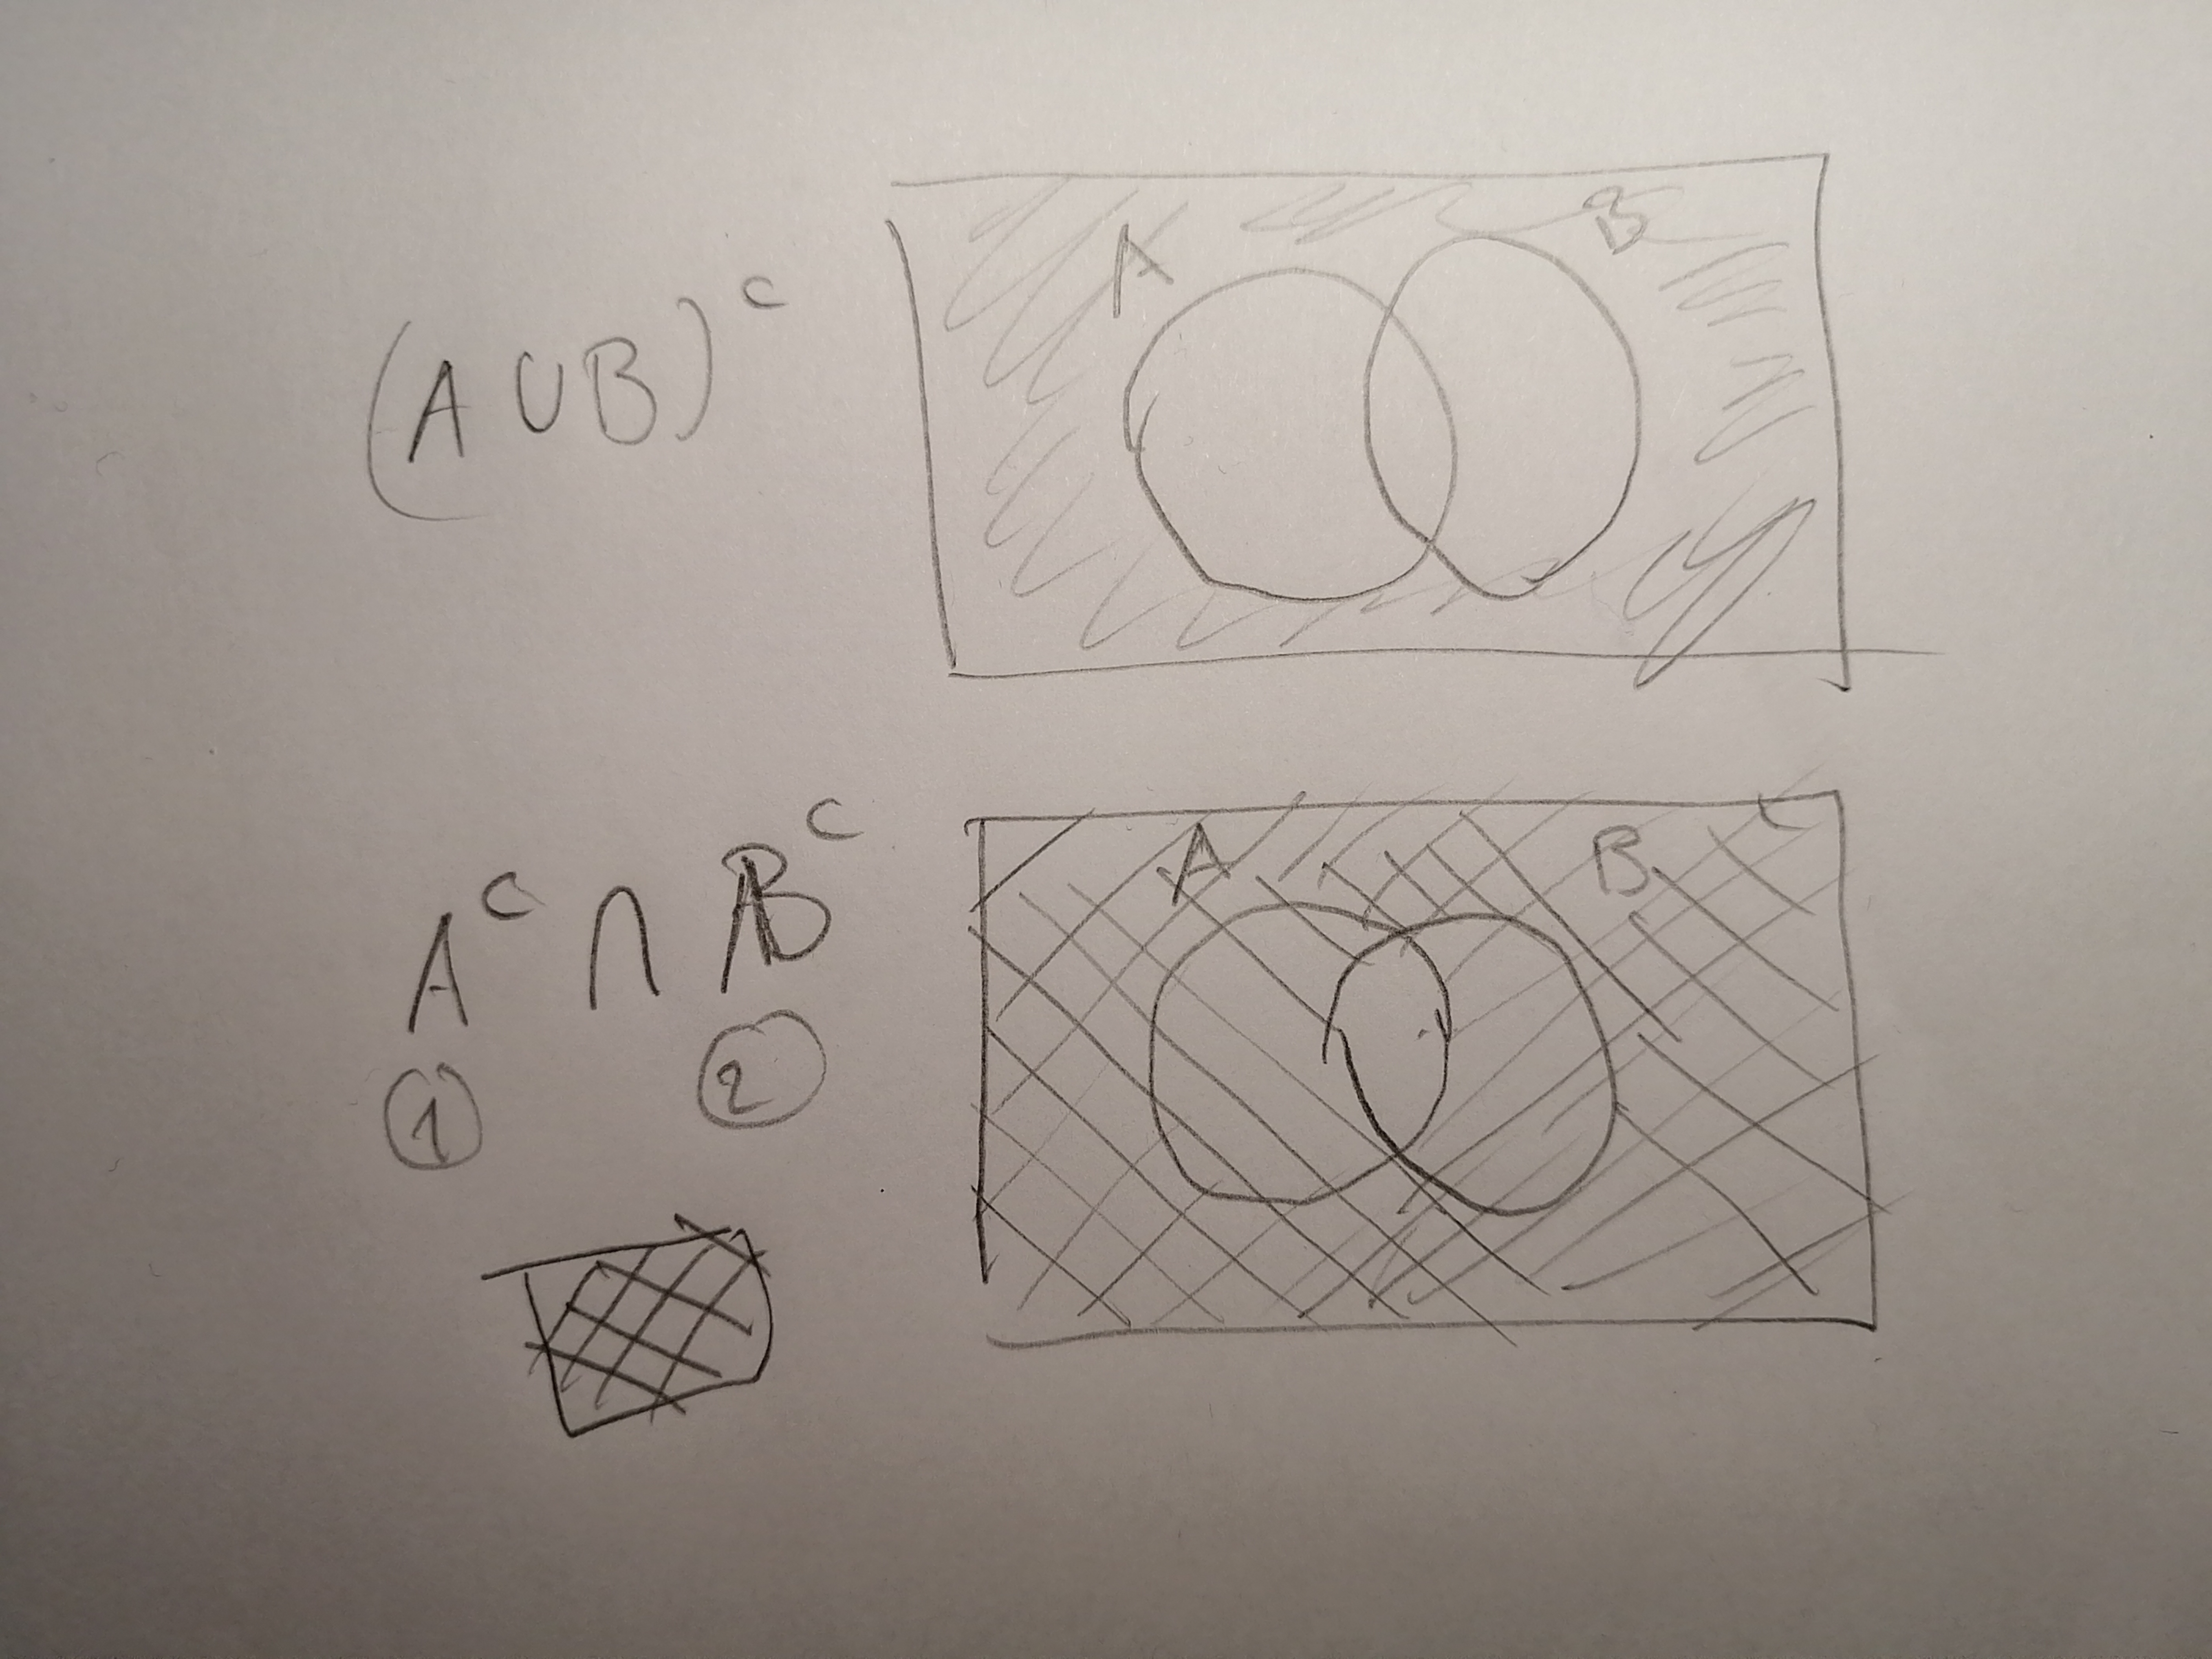
\includegraphics[width=100mm]{assets/dml1.jpg} 
        \end{center}
    \item $\left( A\cap B \right)^{c} = A^{c} \cup B^{c} $, that is not both and and B, is not in A, or not in B or not in either A or B
        \begin{center}
            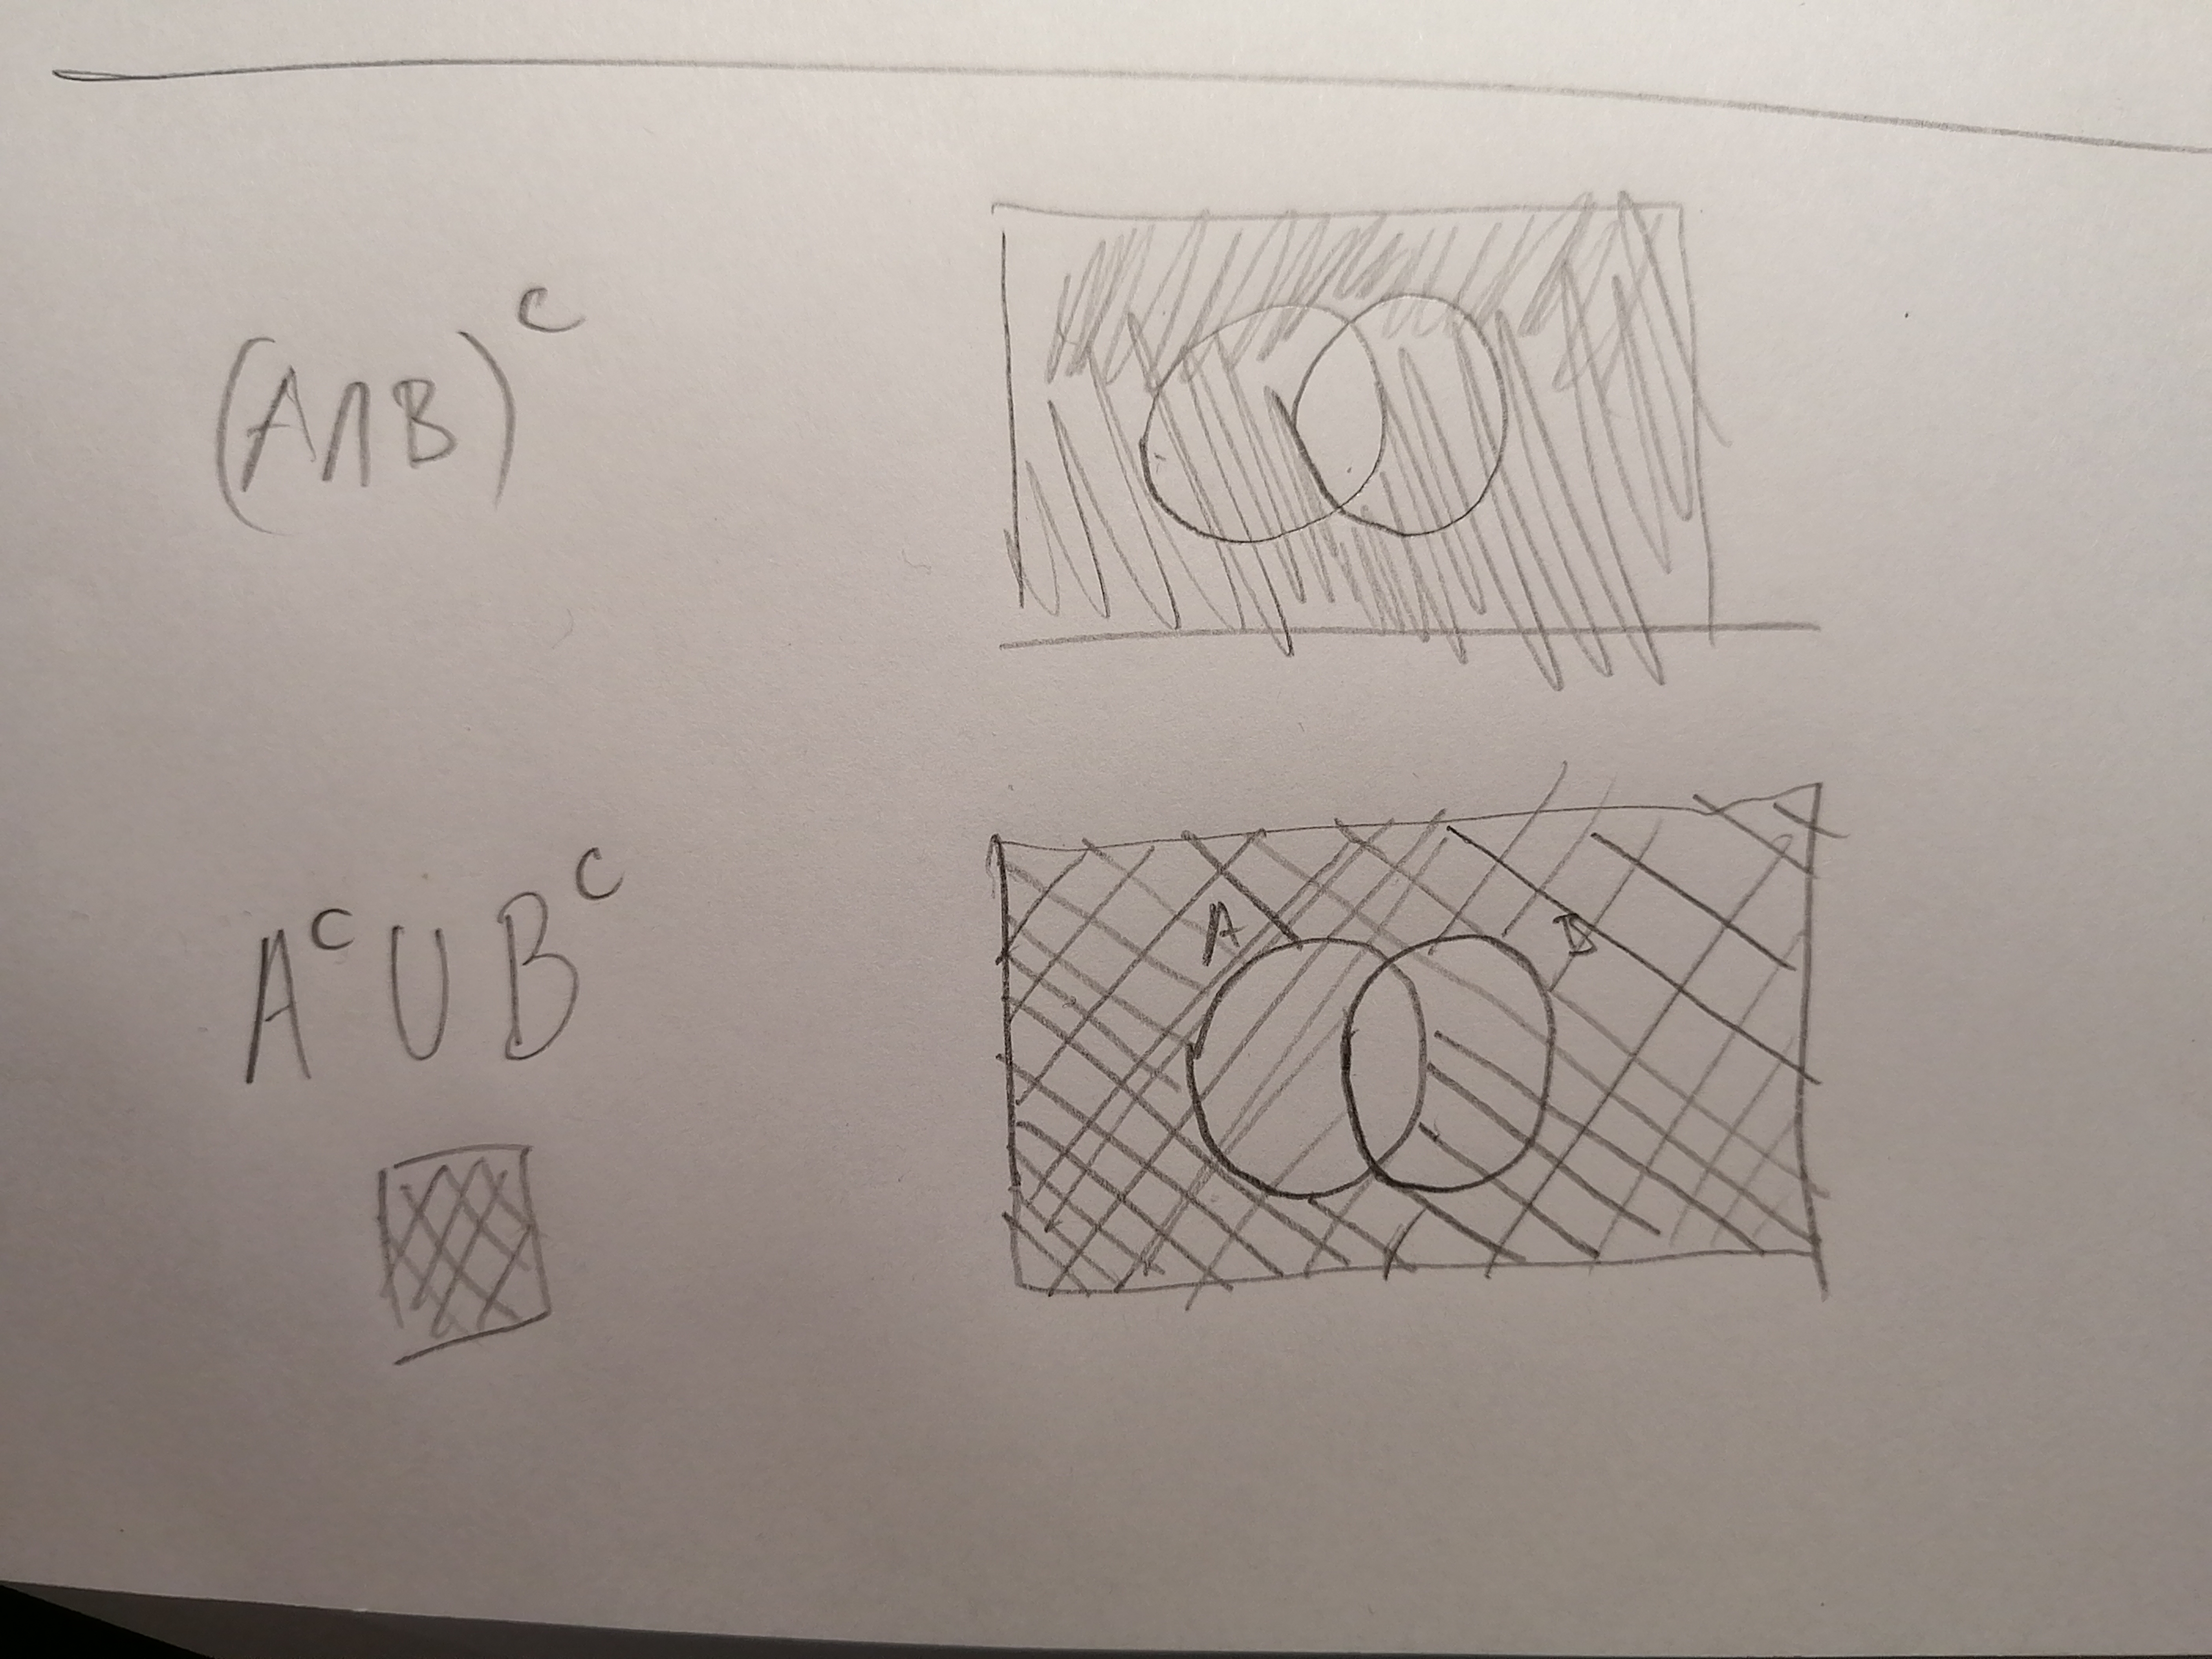
\includegraphics[width=100mm]{assets/dml2.jpg} 
        \end{center}
    The general version we have for set events  $\left\{ A_{1} , A_{2} , \ldots , A_{n}  \right\} $ 
    \begin{itemize}
        \item $\left( \bigcup_{i= 1}^{n} A_{i}  \right) ^{c} = \bigcap_{i=1}^{n} A_{i} ^{c} $ 
        \item $\left( \bigcap_{i=1}^{n} A_{i}  \right) ^{c} = \bigcup_{i=1}^{n} A_{i} ^{c} $ 
    \end{itemize}
\end{itemize}

% section demorgan_s_laws (end)

\section{Sample Space Examples}%
\label{sec:sample_space_examples}
% section sample_space_examples

\begin{enumerate}
    \item Flipping a coin 3 times in a row
        \[
        \Omega = \left\{ HHH, HHT, HTH, HTT, TTT, TTH, THT, THH \right\}  
        \]
        observe that getting two heads, means you also got one tail, therefore $P\left(\text{ Two H } \right) = P\left(\text{ One T } \right) = \frac{3}{8}$ 
    \item Flipping a fair coin 3 times and measuring the number of tails
        \[
        \Omega = \left\{ 0, 1, 2, 3 \right\} 
        \]
        Not all of these are equally as likely, as there are multiple ways of getting just 1 tail, ex, $HHT \text{ and } HTH$ 
    \item Number Selection of an individual's Lotto649 ticket
        \[
            \Omega = \left\{ \left( a,b,c,d,e,f \right) : 1 \le a,b,c,d,e,f \le 49 \in \mathbb{Z}  \right\} 
        \]
        note $n\left(\Omega \right) = 6^{49} $ since there are 49 options for each position
\end{enumerate}

% section sample_space_examples (end)

\section{Event Examples}%
\label{sec:event_examples}
% section event_examples

\begin{enumerate}
    \item Tossing two different dice. The event of tossing a double
        \[
            D= \left\{ \left( 1,1 \right) , \left( 2,2, \right) ,\ldots , \left( 6,6 \right)  \right\} 
        \]
    \item Tossing such that the sum of the two dice is 8
        \[
            S = \left\{ \left( 2,6 \right) ,\left( 3,5 \right) ,\left( 4,4 \right) , \left( 5,3 \right) ,\left( 6,2 \right)  \right\} 
        \]
        observe that the first index of the tuple is the first dice and the second position is for the second dice, therefore $\left( 2,6 \right) \neq \left( 6,2 \right) $ 
    \item Tossing doubles or tossing a sum of 8
        \[
        C= A\cup B 
        \]
    \item Tossing doubles and tossing a sum of 8
        \[
            D= A\cap B= \left\{ \left( 4,4 \right)  \right\} 
        \]
        
\end{enumerate}

% section event_examples (end)

\section{Exclusive \& independence Examples}%
\label{sec:exclusive_&_independence_examples}
% section exclusive_&_independence_examples

\begin{enumerate}[label=\alph*)]
    \item If we know that the course subject is comp sci, then we can assume that the percntage of males will be higher, if we do not know the course subject, then we have no idea, then we don't know if the percentage of males will be higher. Therefore \underline{Dependent}. 
    \item The fact that the coin is baised doesn't matter, every time the coin is tossed, it is still the same probability, therefore getting a head on the first toss tells us nothing about what will happen on the second toss. \underline{Independent} 
    \item If we have someone who doesn't like hiking, then we know that the probability of them climbing mount everest, is lower than just a normal random individual climbing mount everest,therefore by definition it is dependent, though note it is not mutually exclusive since even if they don't like hiking, maybe they want to conquer their fear, so they climb the mountain.
    \item \underline{dependent }, $P\left(\text{ Red Card } \right)= \frac{1}{2} \text{ and } P\left(\text{ Red Card if QoH } \right) = 1$ therefore by definition we know it is dependent . Note if $G$ occurs then , $P\left(\text{ H given G } \right) > \frac{1}{52} $ since one card has been removed
\end{enumerate}

% section exclusive_&_independence_examples (end)

\section{Intro to Probability}%
\label{sec:intro_to_probability}
% section intro_to_probability

\begin{defn}[Probability]\index{Probability}\label{defn:probability}
In a random experiment with sample space $\Omega $,  the \underline{probability} of an event $A$, denoted $P\left(A\right) $ is a function that assigns to event $A$ a numerical value that measures the chance that event $A$ will occur.      
\end{defn}

\subsection{Axioms of Probability}%
\label{sub:axioms_of_probability}
% subsection axioms_of_probability

\begin{enumerate}
    \item $P\left(A\right) \ge 0$ , negative probability doesn't make sense
    \item $P\left(\Omega \right) = 1$,  that is the probability for anything to happen must be 100%
    \item For a set of disjoint events (that is they are mutually exclusive ) $A_{1} , A_{2} , \dotsc  , A_{n - 1} , A_{n} $ in $\Omega $ 
        \[
        P\left(\bigcup_{i=1}^{n} A_{i} \right) = \sum_{i=1}^{n} P\left(A_{i} \right)  
        \]
        this says that probability of any of them happening, is the sum of each probability individually. note this one is very useful for proving things
\end{enumerate}

% subsection axioms_of_probability (end)

\subsection{probability proof}%
\label{sub:probability_proof}
% subsection probability_proof

We'll show the complement relationship
\begin{proof}
    $ $\newline
    Recall $A\cup A^{c} = \Omega $, and $A\cap A^{c} = \emptyset $ , it follows that 
    \begin{gather*}
        P\left(\Omega \right) = P\left(A\cup A^{c} \right) \\
        1= P\left(A\right)  + P\left(A^{c} \right) \\
        P\left(A\right) = 1 - P\left(A^{c} \right) 
    \end{gather*}
\end{proof}

\paragraph{Example} 
If there is a 30\% chance it will rain tommorow, we can conclude that there is a 70\% chance that it will not.

% subsection probability_proof (end)

\section{Inculsion/Exclusion Principle}%
\label{sec:inculsion_exclusion_principle}
% section inculsion_exclusion_principle

We will prove 
\[
P\left(A\cup B\right) = P\left(A\right)  + P\left(B\right)  - P\left(A \cap B\right) 
\]
intuitively, this makes sense as we must subtract what we have double counted.

\begin{center}
    \noindent\rule{8cm}{0.4pt}
\end{center}


Before we continue we will prove a lemma, that is
\[
    P\left(B \cup A^{c} \right) = P\left(B\right)  - P\left(B \cap A\right) 
\]
\begin{center}
    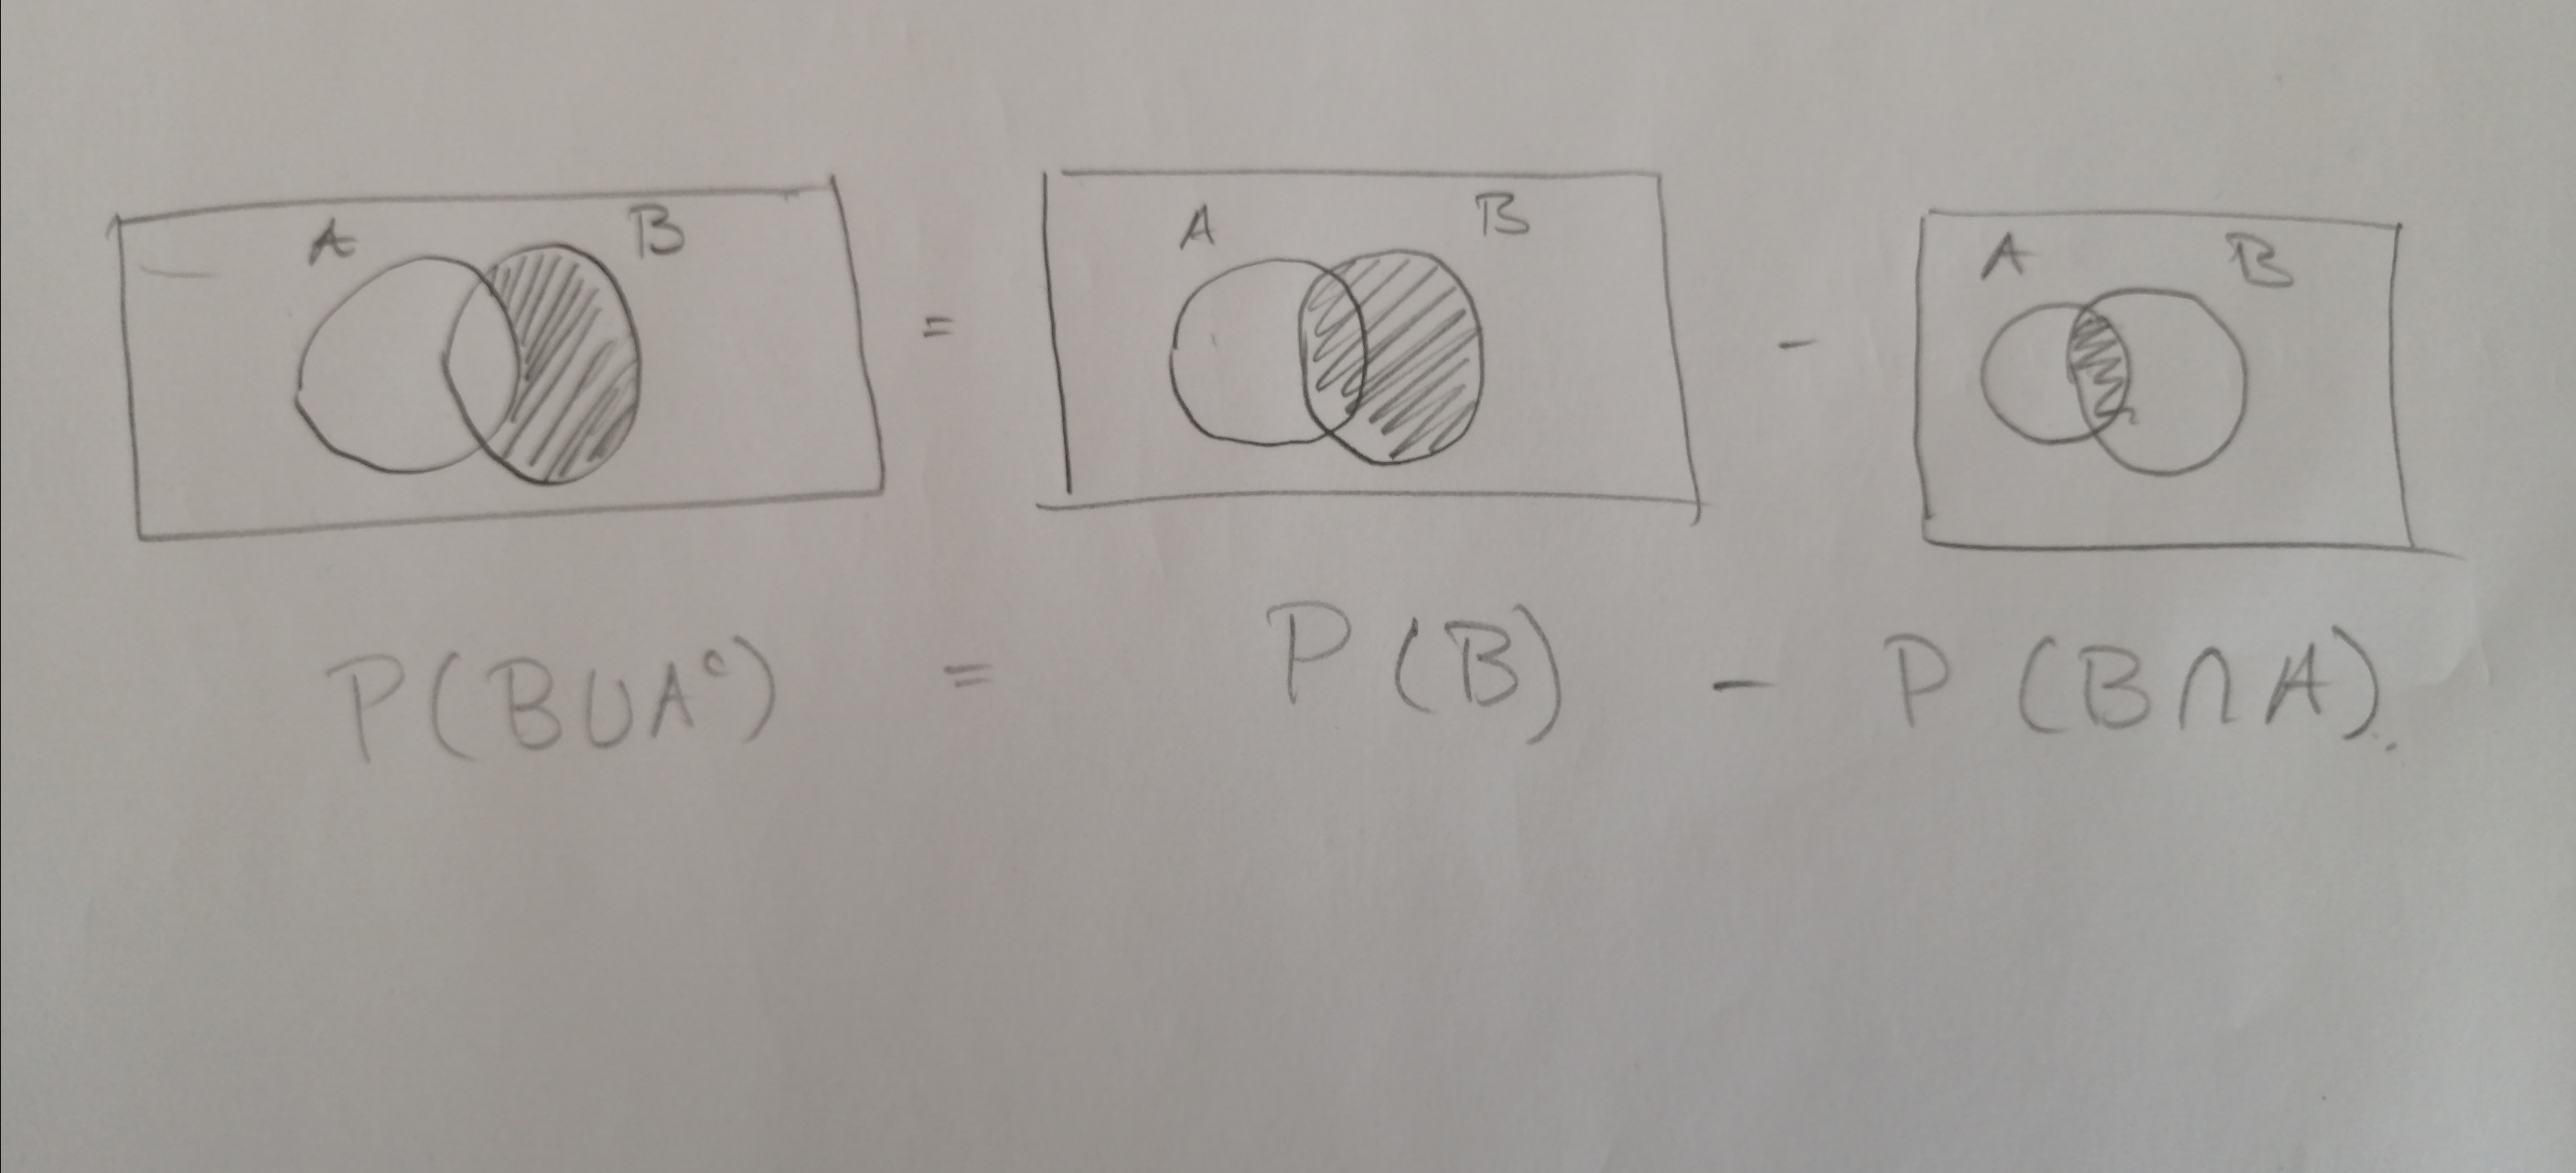
\includegraphics[width=100mm]{assets/p1.jpg} 
\end{center}

Before we continue with the proof, observe the following from above, 
\[
    P\left(\left( B \cup A^{c}  \right) \cup \left( P \cap A \right) \right) = P\left(B\right) 
\]

Though note, that $\left( B \cup A^{c}  \right)\text{ and }  \left( B \cap A \right) $ are disjoint, not proof but visually we can observe it. By axiom 3, we know 
\[
    P\left(B\right) = P\left(\left( B\cup A^{c}  \right) \right)  + P\left(B\cap A\right) \Leftrightarrow P\left(B\cup A^{c} \right) = P\left(B\right)  - P\left(B\cap A\right) 
\]

We will now continue to the main proof 
\begin{proof}
$ $\newline
Observe $A\cup B= A \cup \left( B\cap A^{c}  \right) $ 
\begin{center}
    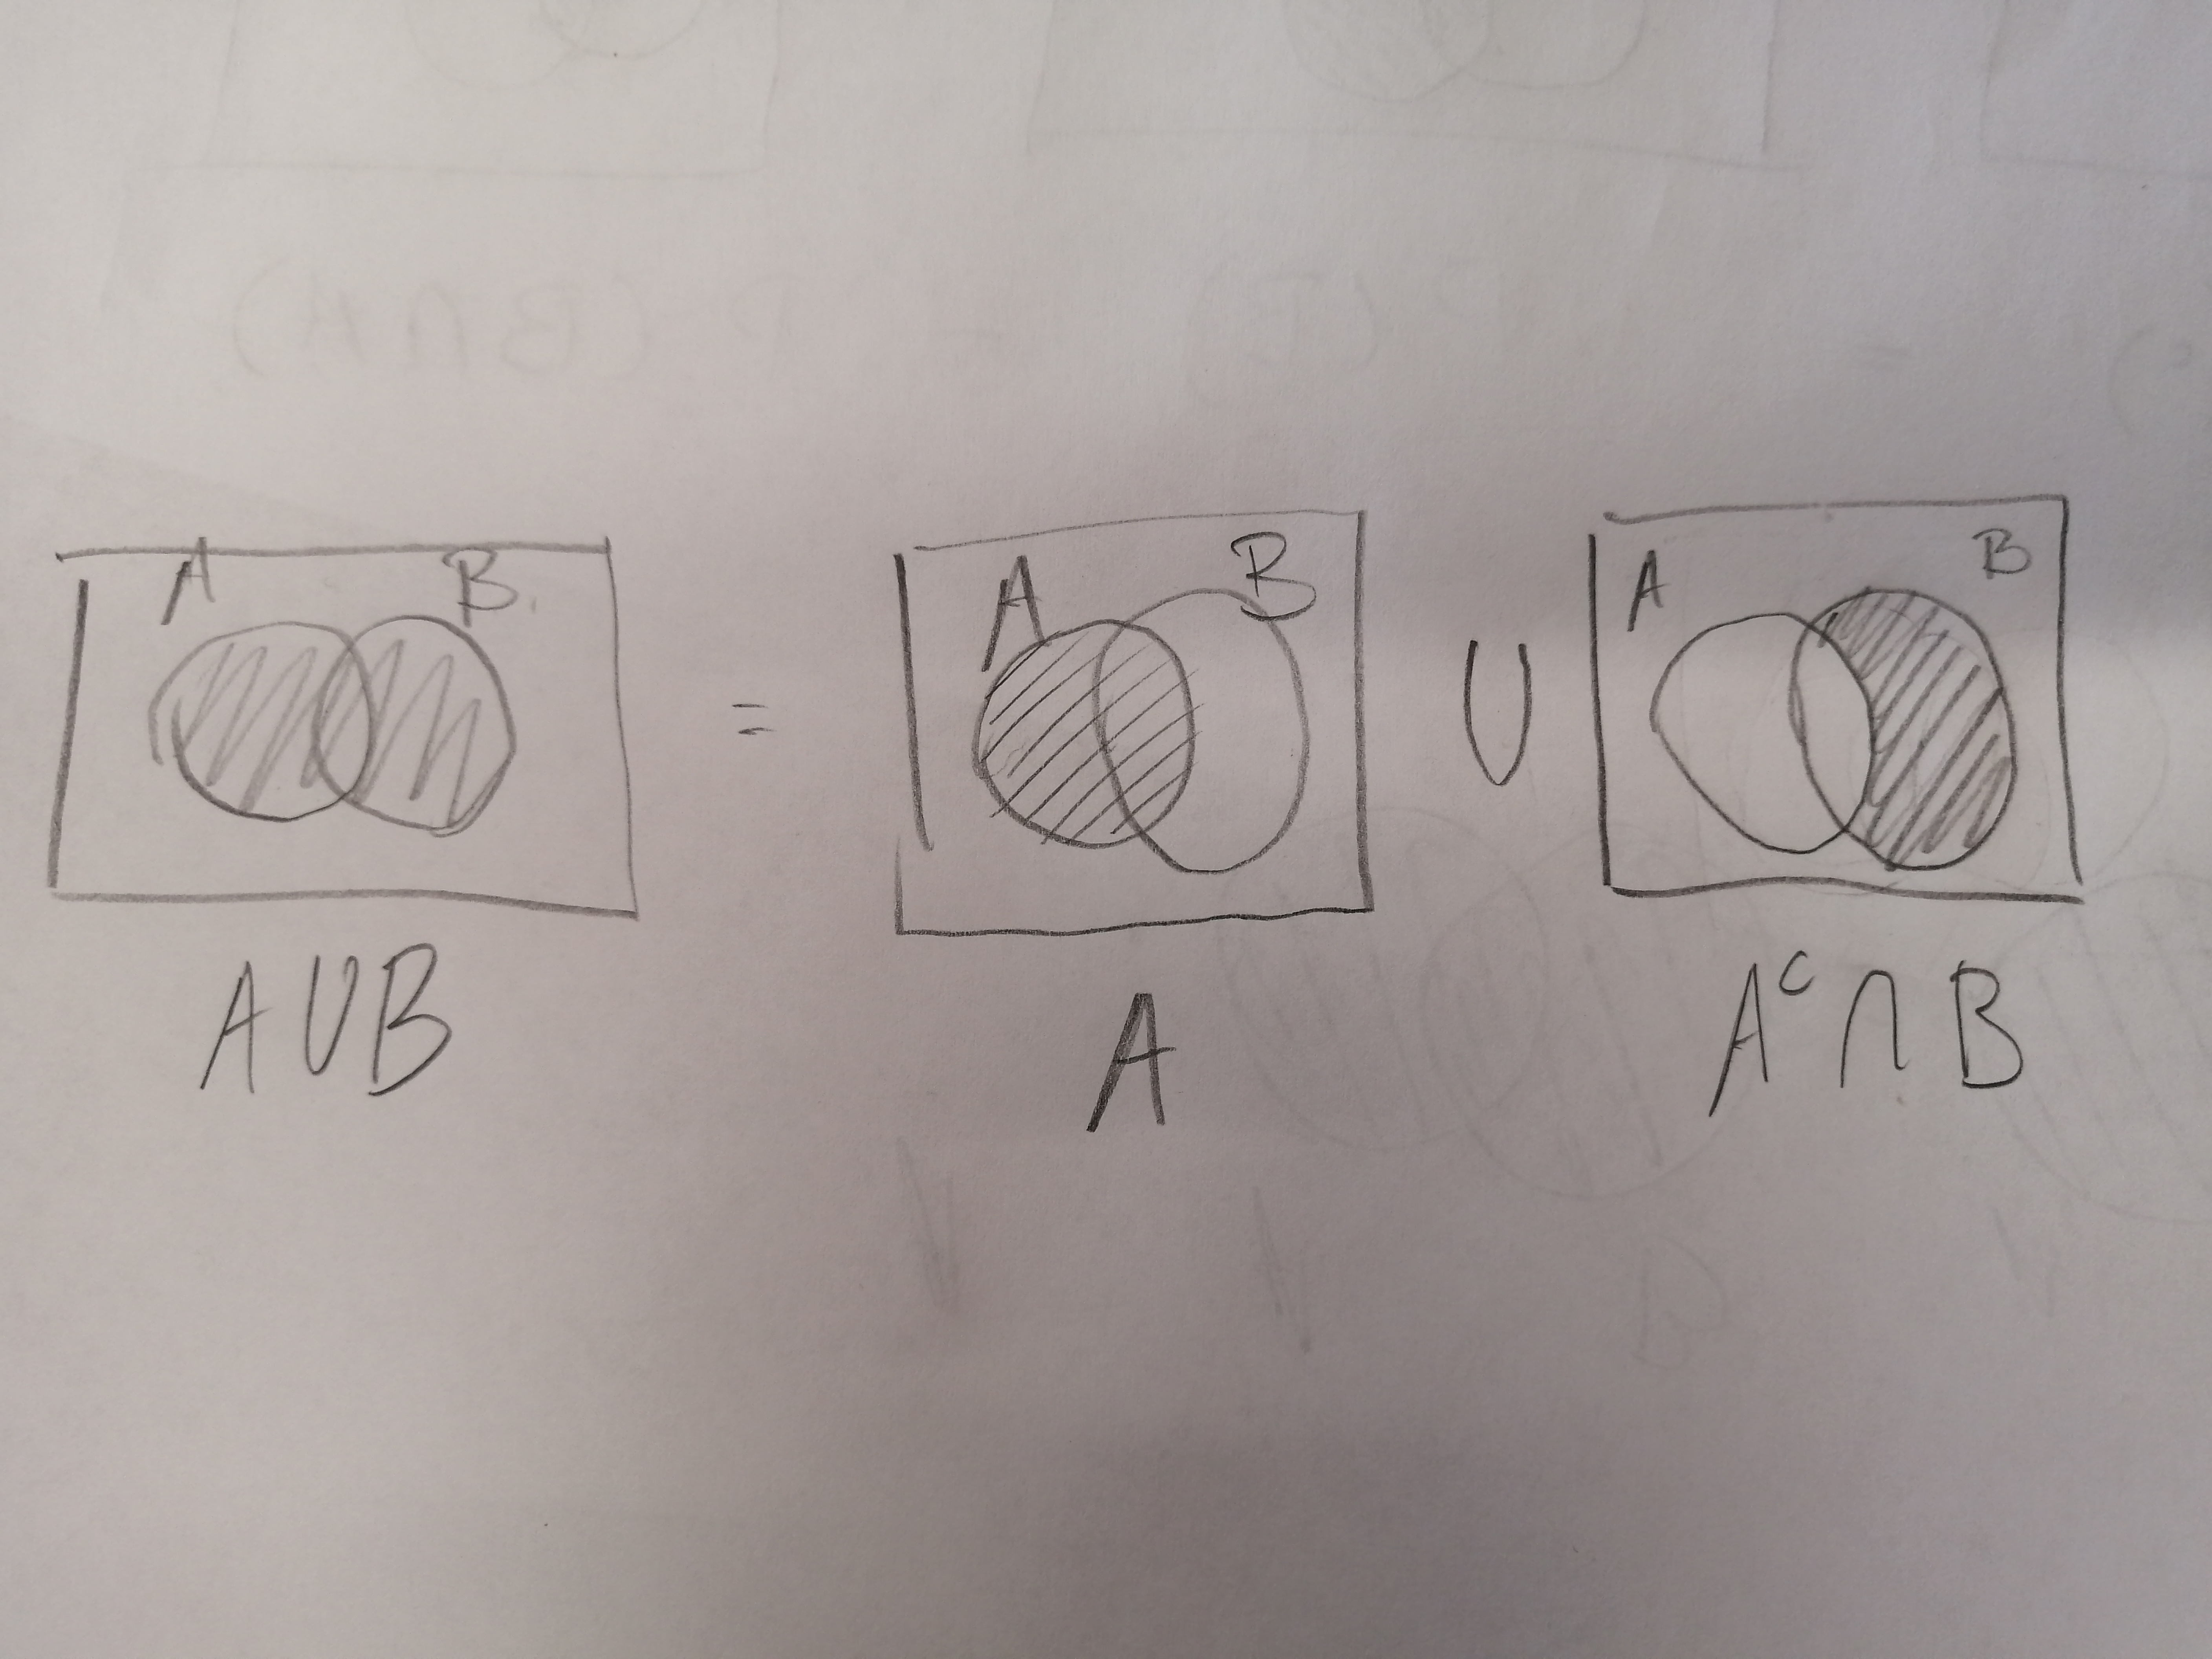
\includegraphics[width=100mm]{assets/ch1_mp.jpg} 
\end{center}
Therefore we know that $A \text{ and } A^{c} \cap B$ are disjoint, it follows that 
\begin{align*}
    P\left(A\cup B\right) &= P\left(A\cup \left( B\cap A^{c}  \right) \right)   \\ 
    &= P\left(A\right)  + P\left(A\cap A^{c} \right) \tag{By axiom 3}  \\ 
    &= P\left(A\right)  + P\left(B\right)  - P\left(A\cap B\right) \tag{By our lemma}
\end{align*}
\end{proof}

\subsection{Triple Example}%
\label{sub:triple_example}
% subsection triple_example

\begin{center}
    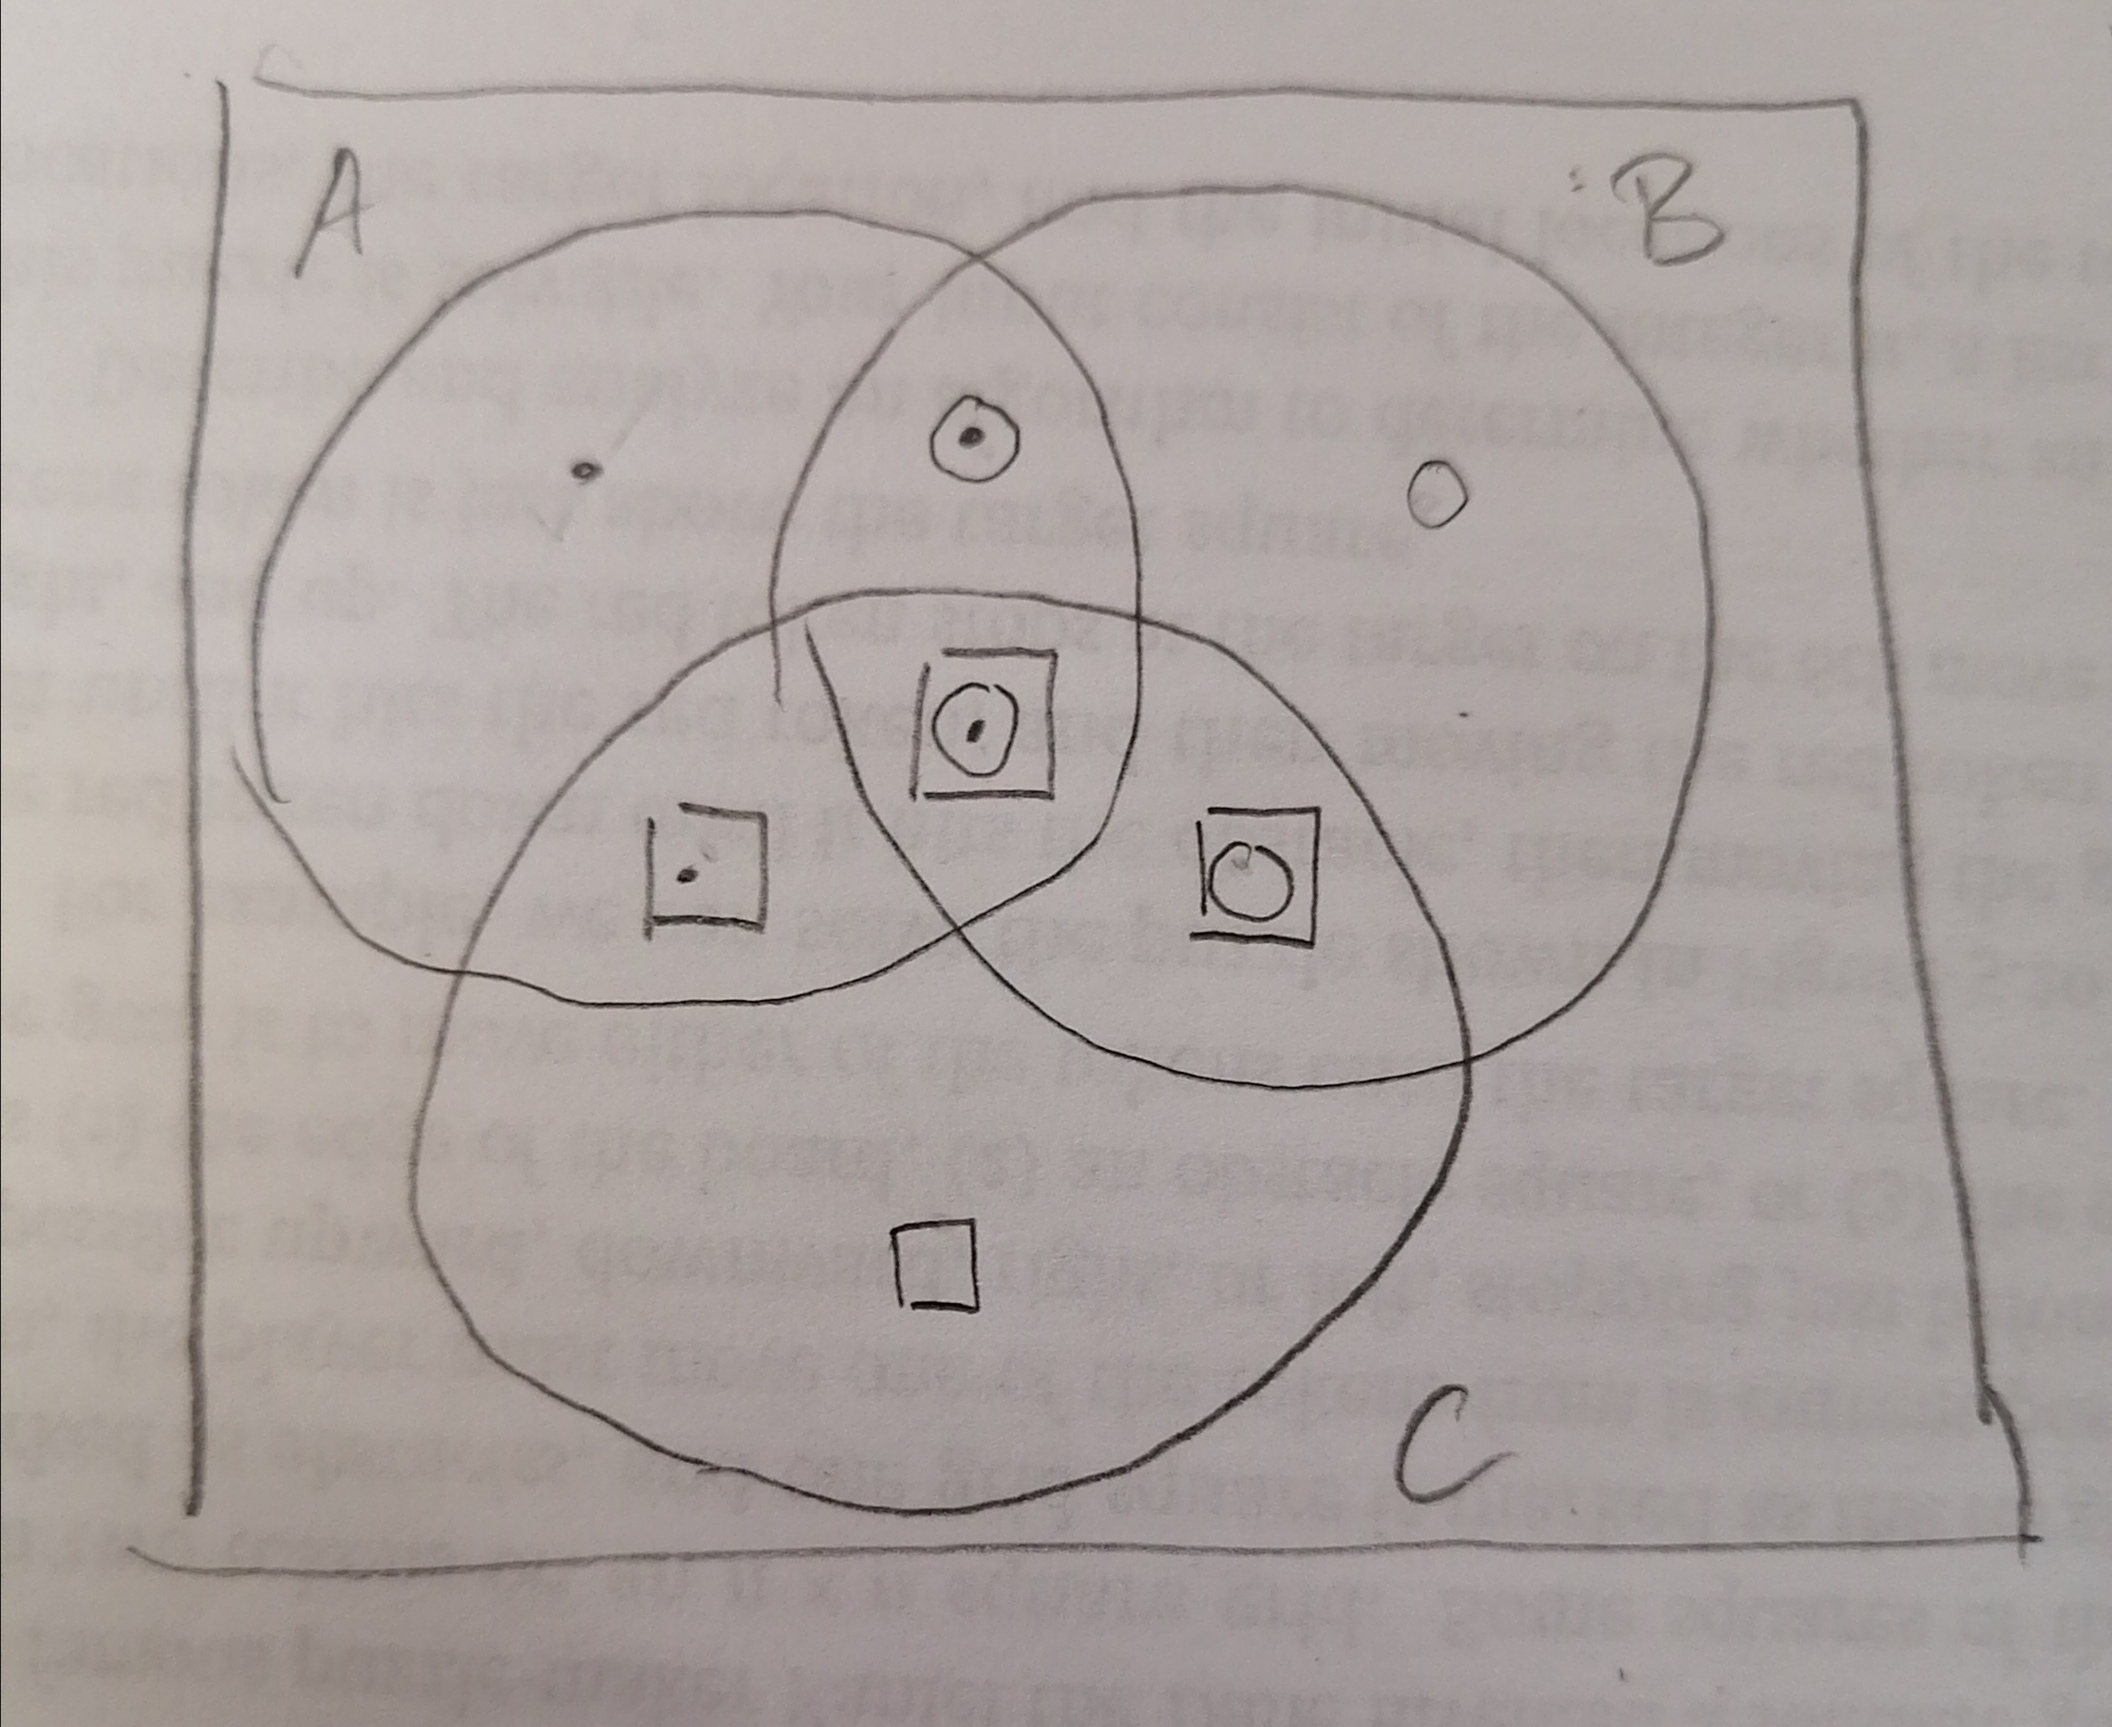
\includegraphics[width=100mm]{assets/lec1_triple.jpg} 
\end{center}

In this example we want to find $P\left(A\cup B\cup C\right) $,  observe  if we find $P\left(A\right)  + P\left(B\right)  + P\left(C\right) $ then clearly we have over counted, but by how much? Let's find out,
\begin{itemize}
    \item From the dots and circles we can see that $A\cup B$ has been double couned.
    \item From the squares and circles, $B\cup C$ has been double counted
    \item From the dots and squares we see that $A\cup C$ has been double counted
    \item Therefore we must subtract both circles from $A\cup B$, both squares from $B\cup C$ and both dots from $C\cup A$ 
\end{itemize}

\begin{center}
    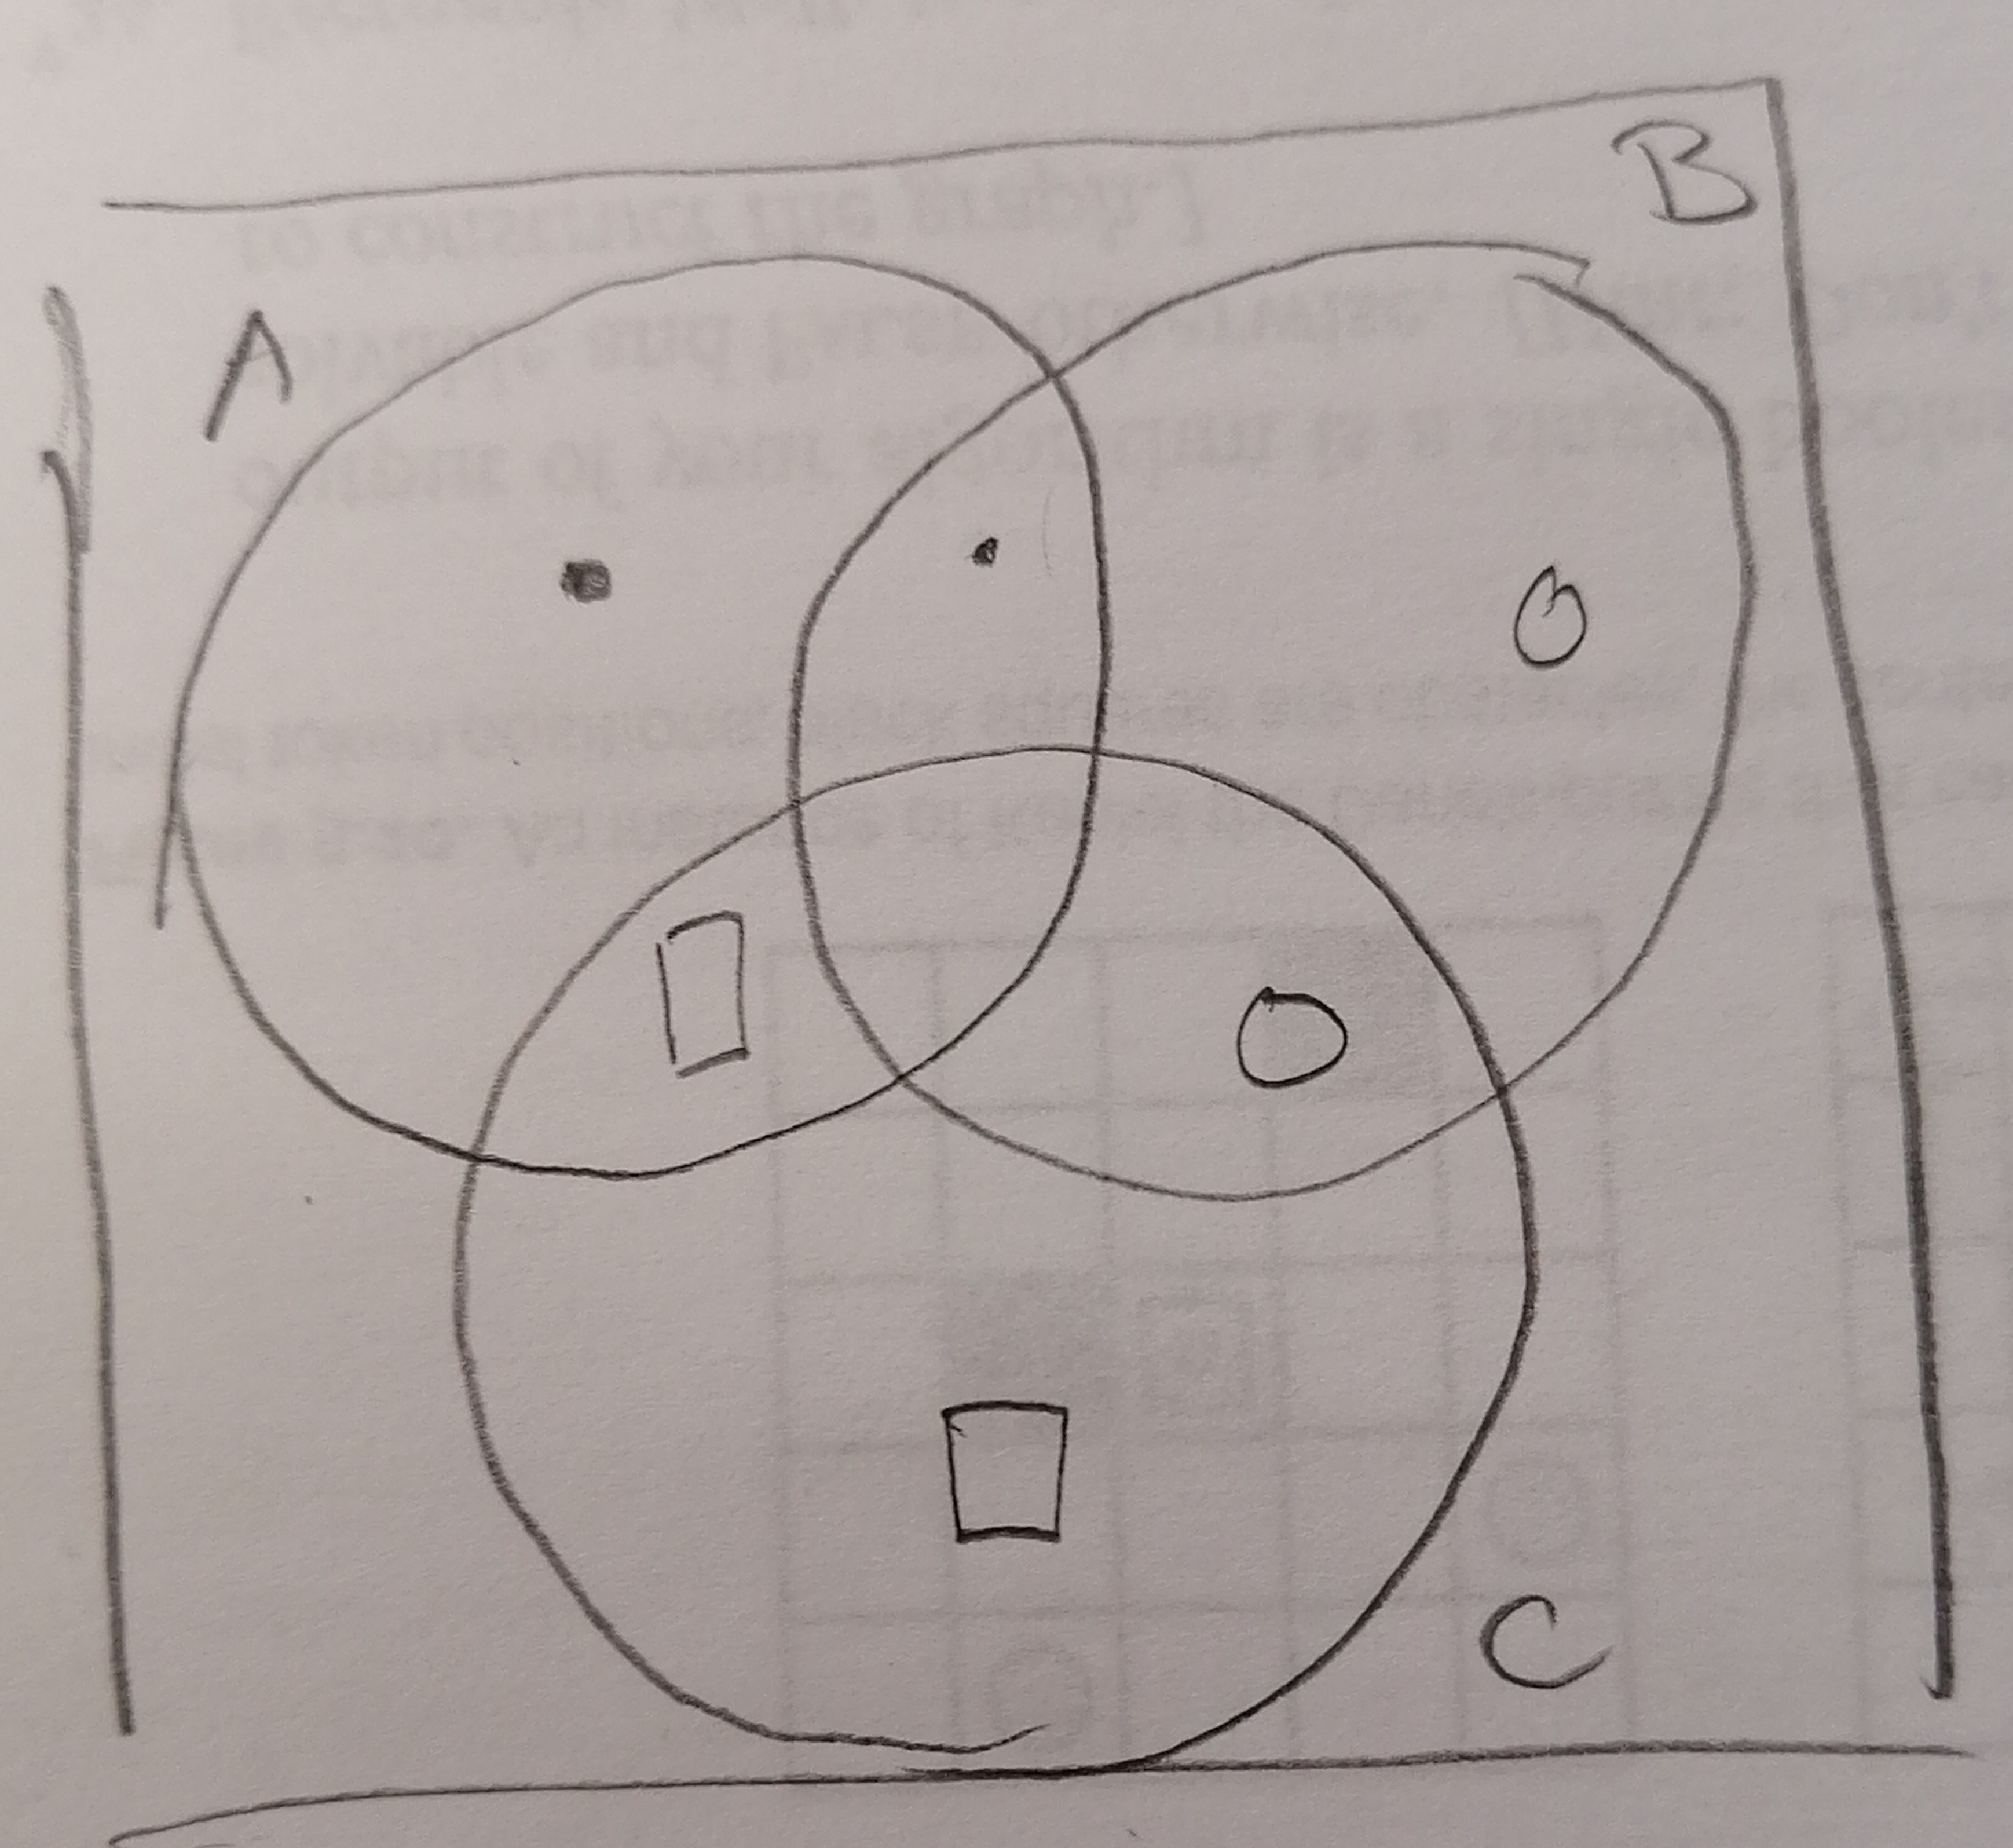
\includegraphics[width=100mm]{assets/lec1_triple_2.jpg} 
\end{center}

After doing so, we see that we have removed all counts of $A\cup B\cup C$ therefore we must add it back, giving us the formula 
\[
P\left(A\cup B\cup C\right) = P\left(A\right)  + P\left(B\right)  + P\left(B\right) - P\left(A\cup B\right)  - P\left(B\cup C\right)  - P\left(C\cup A\right)  + P\left(A\cup B\cup C\right) 
\]

\newpage

Then for $n$ events we get 
\begin{defn}[Inclusion Exclusion Principle]\index{Inclusion Exclusion Principle}\label{defn:inclusion_exclusion_principle}
    \begin{align*}
        P\left(\bigcup_{i=1}^{n} A_{i} \right) &= \sum_{i=0}^{n} P\left(A_{i} \right)  \\
        &- \sum_{1\le i<j \le n}^{n} P\left(A_{i} \cap A_{j} \right)     \\ 
        &+    \sum_{1\le i < j< k \le n} P\left(A_{i} \cup A_{j} \cap A_{k} \right)  \\ 
        &\vdots    \\ 
        &+ \left( -1 \right) ^{n - 1} P\left(\bigcup_{i=1}^{n} A_{i} \right)   
    \end{align*}
\end{defn}

The left hand side is the probability of the union of $n$ events

\begin{itemize}
    \item On the first line of the right hand side we count the probability of being in each set invidually and add it up, though if the sets $A_{i} $ are not disjoint, the some elements have been counted more than once.
    \item therefore on the second line we must subtract anything that was double counted, that is some of the $P\left(A_{i} \cap A_{j} \right) $ may be 0, though if not then we are in fact removing double counts. Since $A_{j} \cap A_{i} = A_{i} \cap A_{j} $ , to avoid duplications we decide to consider only pairs $(A_{i} , A_{j} )$ with $i < j$.
    \item On the previous line we also may have double subtracted though, consider an event who is in $A_{i} \cup A_{j} \cup A_{k} $ it would have been counted for in $A_{i} \cup A_{j} $ in $A_{i} \cup A_{k} $ and $A_{j}\cup  A_{k} $  therefore we add back any elements that had been subtracted more than once
    \item The process contines until the end.
\end{itemize}
% subsection triple_example (end)

\subsection{Inclusion Exclusion Examples}%
\label{sub:inclusion_exclusion_examples}
% subsection inclusion_exclusion_examples

In our class of 200, suppose 87 students had seen Bandersnatch and 45
students had seen Bird Box, while 78 students had watched neither of
these two films. Determine the number of students who...

\paragraph{Watched Both movies} 
\begin{itemize}
    \item Let $A$ be the event of watching Bandersnatch, and $B$ the event of watching Bird Box we want to find the number of people, we need $n\left(A\cap B\right) $ though recall we don't have a formula for that, though we do have one for $n\left(A\cup B\right) $, that is 
        \[
        n\left(A\cup B\right) = n\left(A\right)  + n\left(B\right)  - n\left(A\cap B\right) \Leftrightarrow n\left(A\cap B\right) = n\left(A\right)  + n\left(B\right)  - n\left(A\cup B\right) 
        \]
        We also note that 
        \[
            n\left(A\cup B\right) = 200  - n\left(\left( A\cup B \right) ^{c} \right) = 200  - 78 = 122
        \]
        
        thus we can continue we have 
        \begin{align*}
            n\left(A\cap B\right) &= n\left(A\right)  + n\left(B\right)  - n\left(A\cup B\right) \\
            &= 87 + 45 - 122  \\ 
            &= 132 - 122  \\ 
            &= 10 
        \end{align*}
\end{itemize}

\paragraph{Watched only one of the two movies} 

We want to find the two lunes of $A$ and $B$  on the Venn Diagram, like so
\begin{center}
    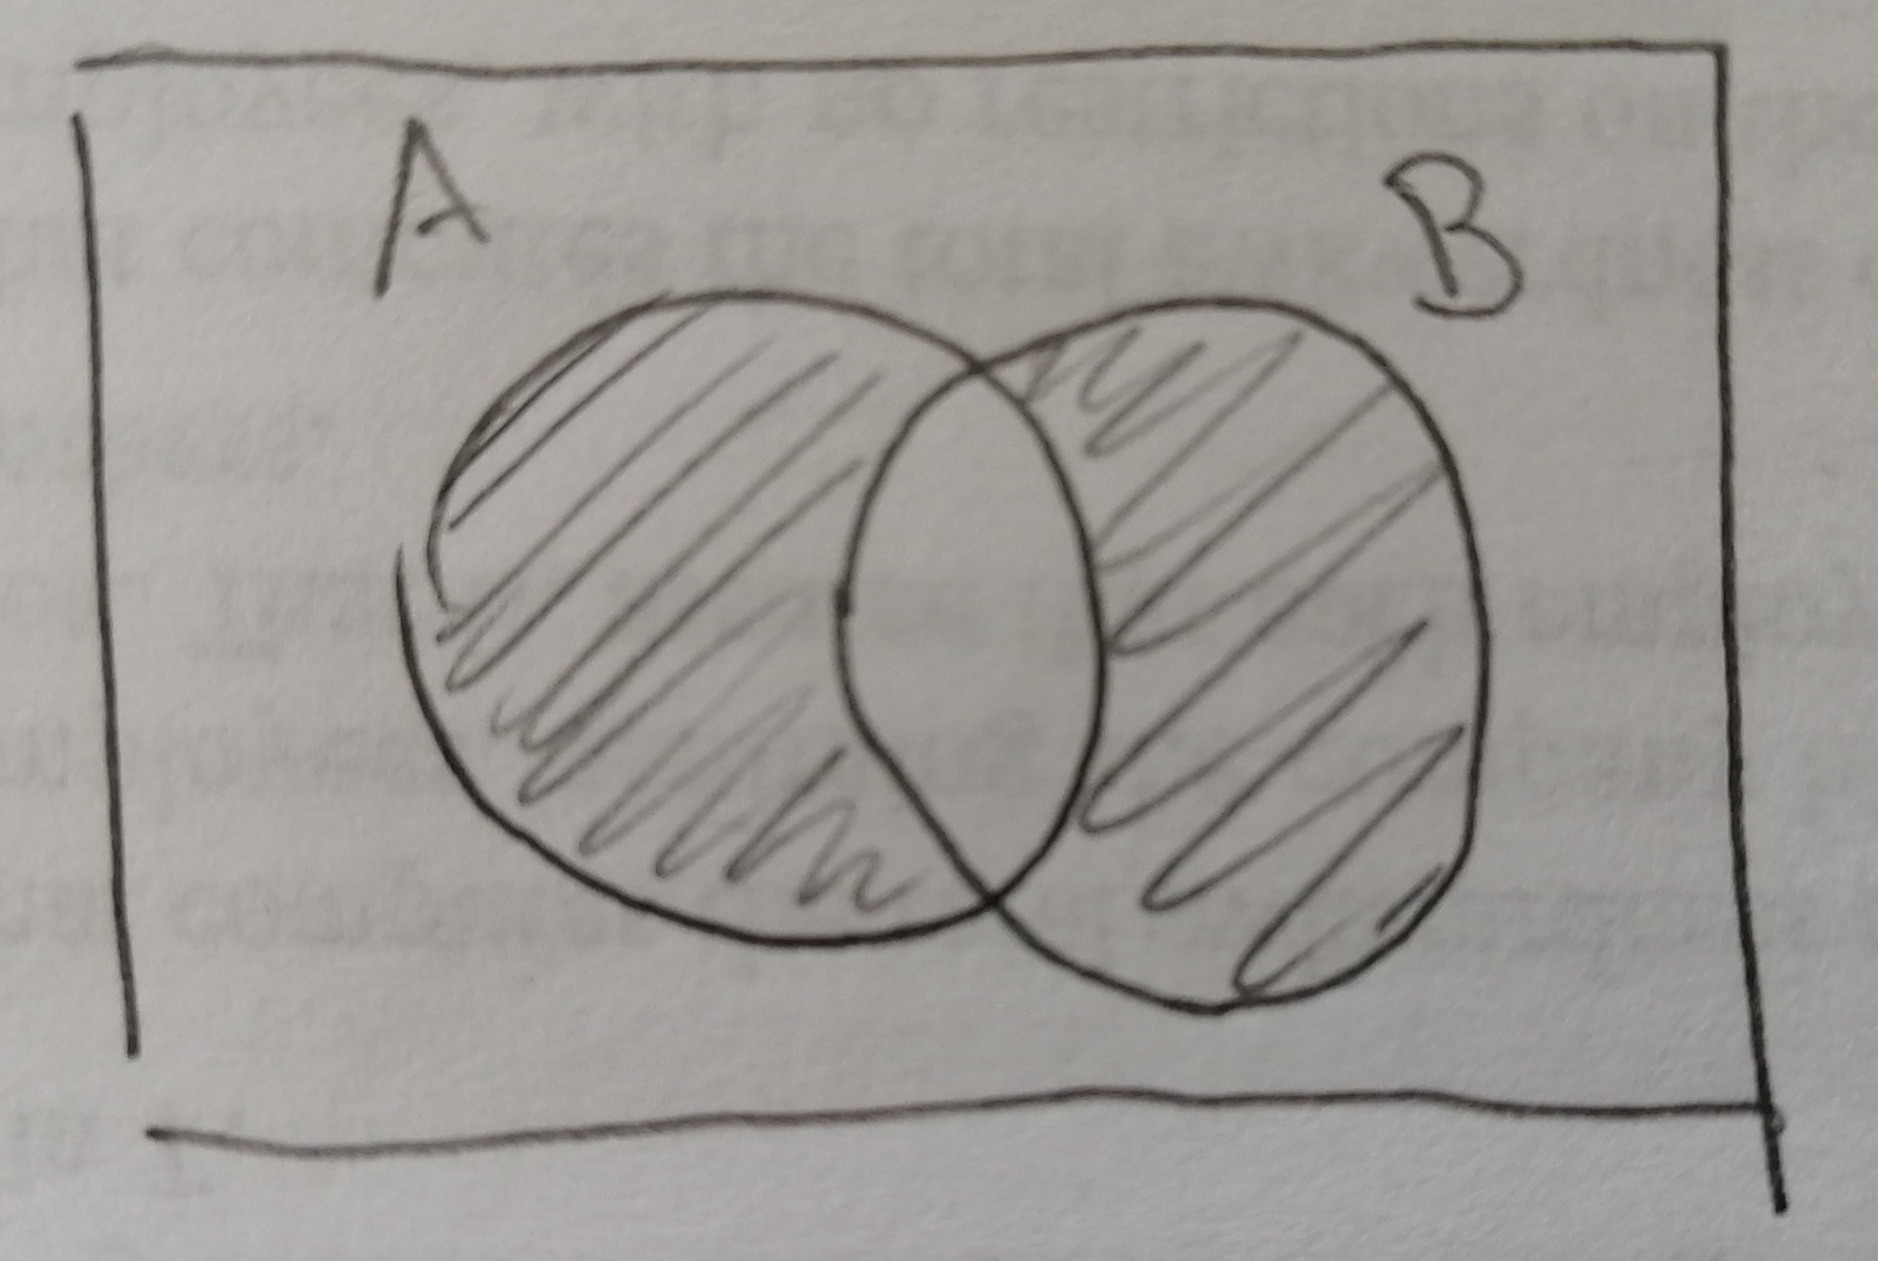
\includegraphics[width=100mm]{assets/lec1_lune.jpg} 
\end{center}

We can write this as $n\left(\left( A^{c} \cap B \right) \cup \left( A\cup B^{c}  \right) \right) $ we observe that they are disjoint therefore we have $n\left(\left( A^{c} \cap B \right) \cup \left( A\cup B^{c}  \right) \right) = n\left(A^{c} \cap B\right)  + n\left(A \cap B^{c} \right) $ 
\begin{itemize}
    \item Note that $n\left(A^{c} \cap B\right) = n\left(B\right)  - n\left(A\cap B\right) $ and $n\left(A\cup B^{c} \right) = n\left(A\right)  - n\left(A\cap B\right) $, so we continue with the calculation to get
        \begin{align*}
            n\left(A^{c} \cup B\right)  + n\left(A\cup B^{c} \right) &= n\left(B\right)  - n\left(A\cap B\right)  + n\left(A\right)  - n\left(A\cap B\right)   \\ 
            &= 45  - 10  + 87  - 10  \\ 
            &= 112  \\ 
        \end{align*}
\end{itemize}

\paragraph{Did not watch Bandersnatch} 
By the completment relation ship we have $n\left(x\right) $ 

% subsection inclusion_exclusion_examples (end)

% section inculsion_exclusion_principle (end)

% section intro_to_probability (end)

% chapter lecture_1 (end)


\end{document}
